%%%%%%%%%%%%%%%%%%%%%%%%%%%%%%%%%%%%%%%%%
% Simple Sectioned Essay Template
% LaTeX Template
%
% This template has been downloaded from:
% http://www.latextemplates.com
%
% Note:
% The \lipsum[#] commands throughout this template generate dummy text
% to fill the template out. These commands should all be removed when 
% writing essay content.
%
%%%%%%%%%%%%%%%%%%%%%%%%%%%%%%%%%%%%%%%%%

%----------------------------------------------------------------------------------------
%	PACKAGES AND OTHER DOCUMENT CONFIGURATIONS
%----------------------------------------------------------------------------------------

\documentclass[12pt]{article} % Default font size is 12pt, it can be changed here

\usepackage{geometry} % Required to change the page size to A4
\geometry{a4paper} % Set the page size to be A4 as opposed to the default US Letter

\usepackage{graphicx} % Required for including pictures

\usepackage{float} % Allows putting an [H] in \begin{figure} to specify the exact location of the figure
\usepackage{wrapfig} % Allows in-line images such as the example fish picture

\usepackage{lipsum} % Used for inserting dummy 'Lorem ipsum' text into the template

\linespread{1.2} % Line spacing

%\setlength\parindent{0pt} % Uncomment to remove all indentation from paragraphs

\graphicspath{{Pictures/}} % Specifies the directory where pictures are stored

\begin{document}
	
	%----------------------------------------------------------------------------------------
	%	TITLE PAGE
	%----------------------------------------------------------------------------------------
	
	\begin{titlepage}
		
		\newcommand{\HRule}{\rule{\linewidth}{0.5mm}} % Defines a new command for the horizontal lines, change thickness here
		
		\center % Center everything on the page
		
		\textsc{\LARGE Wits University}\\[1.5cm] % Name of your university/college
		\textsc{\Large School of Electrical and Information Engineering}\\[0.5cm] % Major heading such as course name
		\textsc{\large ELEN7046 - Software Technologies and Techniques}\\[0.5cm] % Minor heading such as course title
		
		\HRule \\[0.4cm]
		{ \huge \bfseries Big Data Visualization using Commodity Hardware and Open Source Software}\\[0.4cm] % Title of your document
		
		\HRule \\[0.6cm]
		
		\begin{minipage}
			{0.4
				\textwidth} 
			\begin{flushleft}
				\large \emph{Authors:}\\
				Gareth \textsc{Stephenson} \\
				Matsobane \textsc{Khwinana} \\
				Sidwell \textsc{Mokhemisa} \\
				Dave \textsc{Cloete}\\
				Kyle \textsc{Trehaeven}
			\end{flushleft}
		\end{minipage}
		~ 
		\begin{minipage}
			{0.4
				\textwidth} 
			\begin{flushright}
				\large \emph{Student Number:} \\
				778919 \\
				779053  \\
				1229756 \\
				1573016 \\
				0602877N
				% Supervisor's Name
			\end{flushright}
		\end{minipage}
		\\[1cm]
		
		% Abstract
		\begin{flushleft}\large
			\textsc{Abstract}\\
			The project aims to provide a low cost solution to big data processing problems, enabling a commercially viable option to individuals, small businesses and academia using commodity hardware. This report explores the use of  Open Source technologies Apache Spark and Scala as well as the low cost and scalable Raspberry Pi's. After building a prototype system to source, process and visualize data from twitter, it was concluded that  commodity hardware is a viable small-scale solution to working with Big Data.
			
		\end{flushleft}
		{\large \today}\\[3cm] % Date, change the \today to a set date if you want to be precise
		
		%\includegraphics{Logo}\\[1cm] % Include a department/university logo - this will require the graphicx package
		
		\vfill % Fill the rest of the page with whitespace
		
	\end{titlepage}
	
		% Abstract
		\begin{flushleft}\large
			\textsc{Declaration of Originality}\\
			
			
		\end{flushleft}
	
	%----------------------------------------------------------------------------------------
	%	TABLE OF CONTENTS
	%----------------------------------------------------------------------------------------
	
	\tableofcontents % Include a table of contents
	
	\newpage % Begins the essay on a new page instead of on the same page as the table of contents 
	
	%----------------------------------------------------------------------------------------
	%	INTRODUCTION
	%----------------------------------------------------------------------------------------
	
	\section{Introduction} % Major section
	
This report presents the work done by Group 2 in response to the project brief for ELEN7046: Software Technologies and Techniques.\\

The report will broadly focus on the following topics:

\begin{itemize}
	\item The Methodology followed to execute the project;
	\item The Architecture of the solution developed for the project; and
	\item The different technologies used to deliver the solution.
\end{itemize}

\subsection{Problem Statement}

There is an abundance of big data available to individuals and companies with very limited capacity to refine this data into meaningful information, particularly for small scale endeavours. Big Data processing is often locked behind high cost barriers to entry, and individuals, start ups and academics may find it difficult to be involved in Big Data processing.

\subsection{Solution Summary}

Commodity hardware is available to provide a means by which the barrier to entry for Big Data projects can be overcome. Simple, low cost components can be leveraged to address each of the parts of a big data processing solution, whether it be data sourcing, transormation, or visualization; and can be scaled according to needs or as required.

\subsection{Approach}

%\subsubsection{Methodology}
	
		%\subsection{Executive Summary} % --optional
		
		%------------------------------------------------
		
	\section{Literature Review}
	
	\subsection {Data Sourcing}
	
	This project was intended to deliver a system or solution for the visualization of Big Data. For this reason it is important that we start by defining what Big Data is.
	\\
	According to Maden[1], Big Data can be defined as "data that is too big, too fast, or too hard for existing tools to process."
	\\
	The above definition further supports our group's decision to focus on Twitter as the source of data for the project. Statistics have shown the following average figures with regards to the amount of data that one can get from Twitter[2]:
	\\
	
		\begin{itemize}
			\item 6000 per second; 
			\item 350 000 per minute;
			\item 500 million per day; and
			\item 200 billion in a year.
		\end{itemize}
	
	\subsection {Big Data Processing Algorithm}
	
	The team sought to have all the processing of the Big Data received from Twitter done on multiple nodes following the principles of MapReduce.
	\\
	\\
	Apache Spark was used for this project together with MapReduce which in the main delivers the MapReduce functionality based on the algorithm that is broken down into the Mapper class and the Reducer class[3].

		%--Where they come from
		%--What they currently do
		%--General experience
	
	%Example citation \cite{Figueredo:2009dg}.
	
	%------------------------------------------------
	
	%\subsection{Description of Acronyms} % Sub-section
	
	%IS - Information Systems \\
	
	%------------------------------------------------
	%Sample image for future reference (image to be taken out)
	%\begin{figure}[H] % Example image
	%\center{
\includegraphics[width=0.5\linewidth]{placeholder}}
	%\caption{Example image.}
	%\label{fig:speciation}
	%\end{figure}
	
	%------------------------------------------------
	%-------------
	%	MAJOR SECTION 1
	%----------------------------------------------------------------------------------------
	
	%\section{Problem Statement}
	
	
	
	%\subsection{Executive Summary} % --optional
	
	%------------------------------------------------
	
%	\subsection{Data Collection}
	%--Where they come from
	%--What they currently do
	%--General experience
	
	
	
	%------------------------------------------------
	
%	\subsection{Data Processing}
	


	%--Risk categories SP03
	
%	\subsubsection{Cost and Schedule}
	
	
	
	%--Earn Value Management SP01
	
	
	%--Earn Value Management SP01
	
%	\subsection{Data Visualization}
	

	%--Summary of the above
	%--Kill project/replace project manager/continue project???
	
	%------------------------------------------------
	
	\section{Lifecycle Methodology}
	
	%\subsection{Explanation Summary} %--optional
	
	%------------------------------------------------
	In order for the team to successfully deliver this project, a development methodology based on IBM Rational Unified Process (RUP) was followed albeit tailored to cater for the specific needs of this project.\\
	\\
	The diagram below depicts the IBM RUP model:
	
		\begin{figure}[H] % Example image
			\center{\includegraphics[width=1.15\linewidth]{ibm1}}
			\caption{IBM Rational Unified Process (Source: RUP, Best Practices for Software Development Teams)}
			\label{fig:speciation}
		\end{figure}
		
		
	
%	\subsection{info}
	
	
	%------------------------------------------------
	
%	\subsection{Observation} % Sub-section
	
	
%	\subsubsection{Value}
	
	
	%\\subsubsection{Risk}
	%--Risk categories SP03

%	\subsubsection{Cost \& Schedule}
	

	
	%\subsection{xxx}
	\section{Assumptions and Constraints}
	
		\subsection{Tweet Locations}
		The group encountered tweet location issues. \\
		\subsection{Pros and Cons determinations}
		Rudimentary algorithm for determining Twitter statements (tweets) that are against or for a particular candidate was adopted... \\
	
	%------------------------------------------------
	\section {Design Decisions}
	
	The table below details all the key design decision made in the delivery of the solution:
	\\
	
\begin{itemize} 
	\item \textbf{History Data:} History data/ batch interface to Twitter was designed to provide past data subscribed to based on date range.
	
	\item \textbf{Streaming Data:} 
	This interface provides for all subscribed data in real-time starting from now and going into the future.
	
	\item \textbf{GoogleMaps:} 
	Tweet location was derived from the co-ordinates found in a tweet where the person tweeting enabled location services on their device to provide current location information. Where privacy settings were not enabled for current location, an interface to GoogleMaps was developed to read the location information of the person tweeting from their Twitter profile and resolve this to actual co-ordinates.
	
	\item \textbf{Security Directive(s):} 
	It was decided that where security is concerned, only the Twitter and GoogleMaps security requirements be adhered to where integration is concerned. All data acquired from Twitter is data that is already in the public domain, therefore no effort was required to secure the data while in transit, hence the use of only FTP instead of a lot more secure transport mechanism.
\end{itemize}
	
	
	
	%\subsection{Explanation Summary} %--optional

	%------------------------------------------------
	
	%--Earn Value Management 
	
	
	%--Summary of the above
	%--Kill project/replace project manager/continue project???

	
	
	%-----------------------------------------------
	
	\section{Success Criteria} % Major section
	
	\begin{itemize}
		\item Build a system that uses commodity hardware to solve for big data problems;
		\item Provide a solution that covers the data sourcing, transformation and presentation of social media data from Twitter relating to the United States and South African elections. The end result must be visualization that provides insight to the sentiment of election candidates on Twitter.
	\end{itemize}
	
	
	
	\section{Solution Design}
		
	\subsection{High Level Design: Component Architecture}
	
	
		\begin{figure}[H] % Example image
			\center{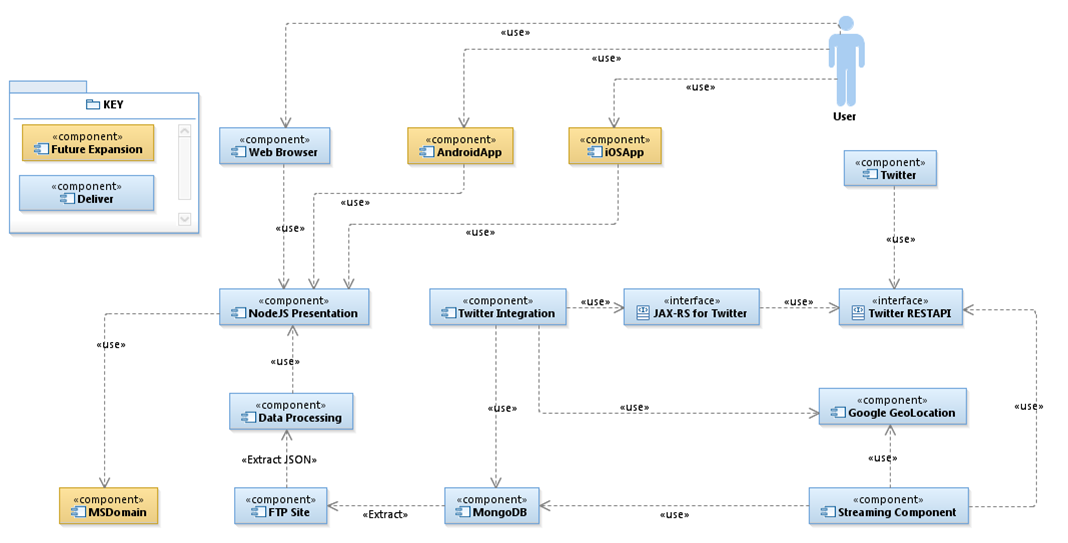
\includegraphics[width=1.15\linewidth]{HLD1}}
			\caption{High Level Component Model.}
			\label{fig:speciation}
		\end{figure}
	
	\subsection{Detailed Designs}
	
	\subsubsection{Data Acquisition (Batch)}
	
		\begin{figure}[H] % Example image
			\center{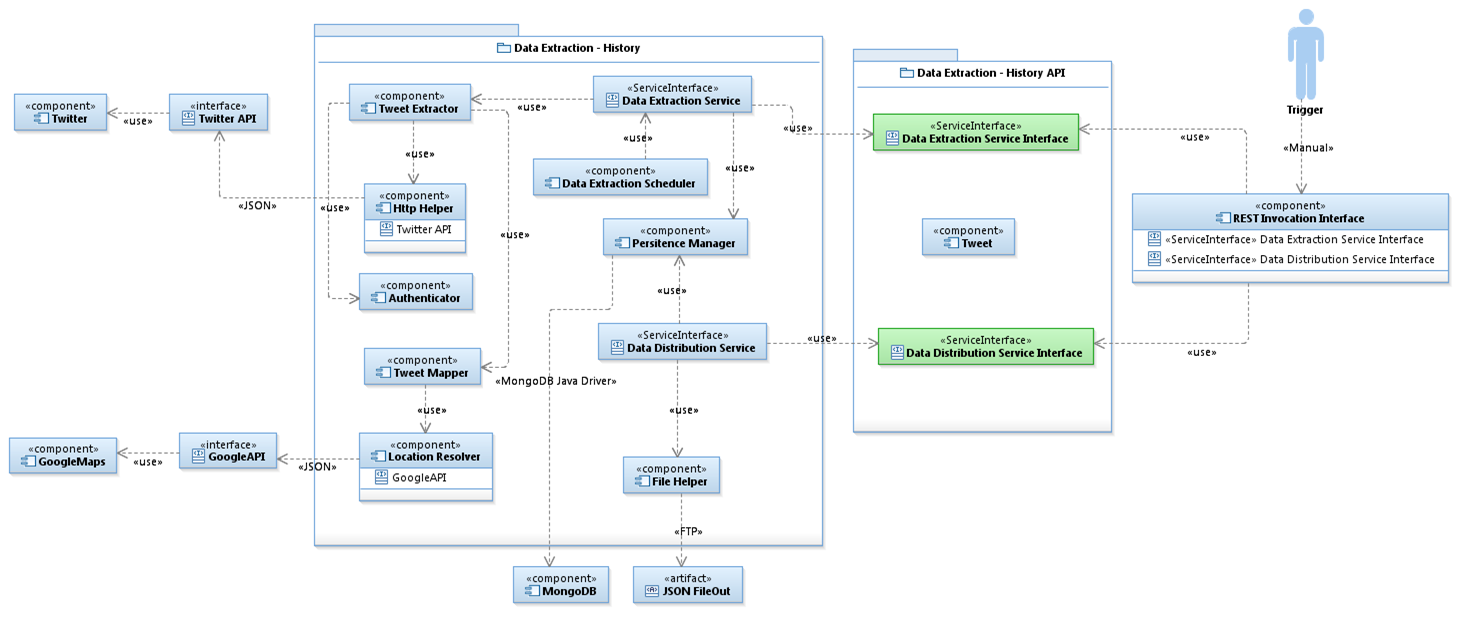
\includegraphics[width=1.15\linewidth]{Batch}}
			\caption{Component Model: Streaming Module}
			\label{fig:speciation}
		\end{figure}
	
	\subsubsection{Data Acquisition (Streaming)}
	
		\begin{figure}[H] % Example image
			\center{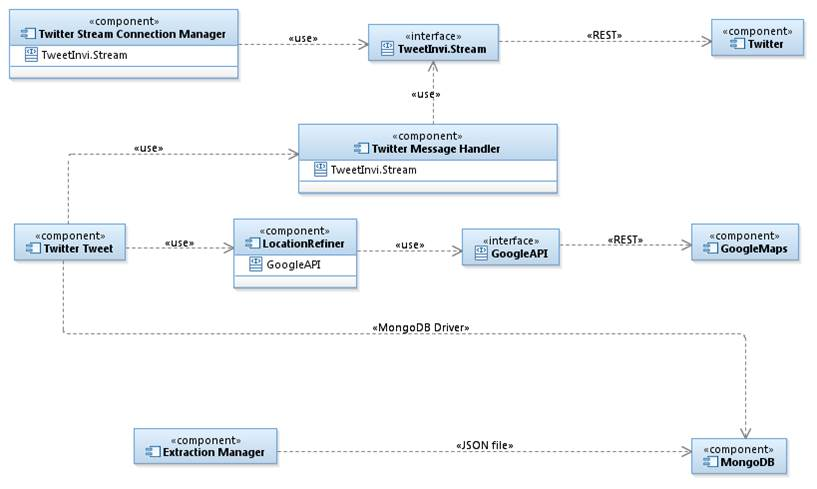
\includegraphics[width=1.15\linewidth]{Streaming}}
			\caption{Component Model: Streaming Module}
			\label{fig:speciation}
		\end{figure}
	
	\subsubsection{Data Processing}
	
	\begin{figure}[H] % Example image
		\center{\includegraphics[width=1.15\linewidth]{MapReduce}}
		\caption{Context Diagram: Data Processing}
		\label{fig:speciation}
	\end{figure}
	
	\subsubsection{Data Visualization}
	
	\subsection{Operational Model: Infrastructure Design}
	
		\begin{figure}[H] % Example image
			\center{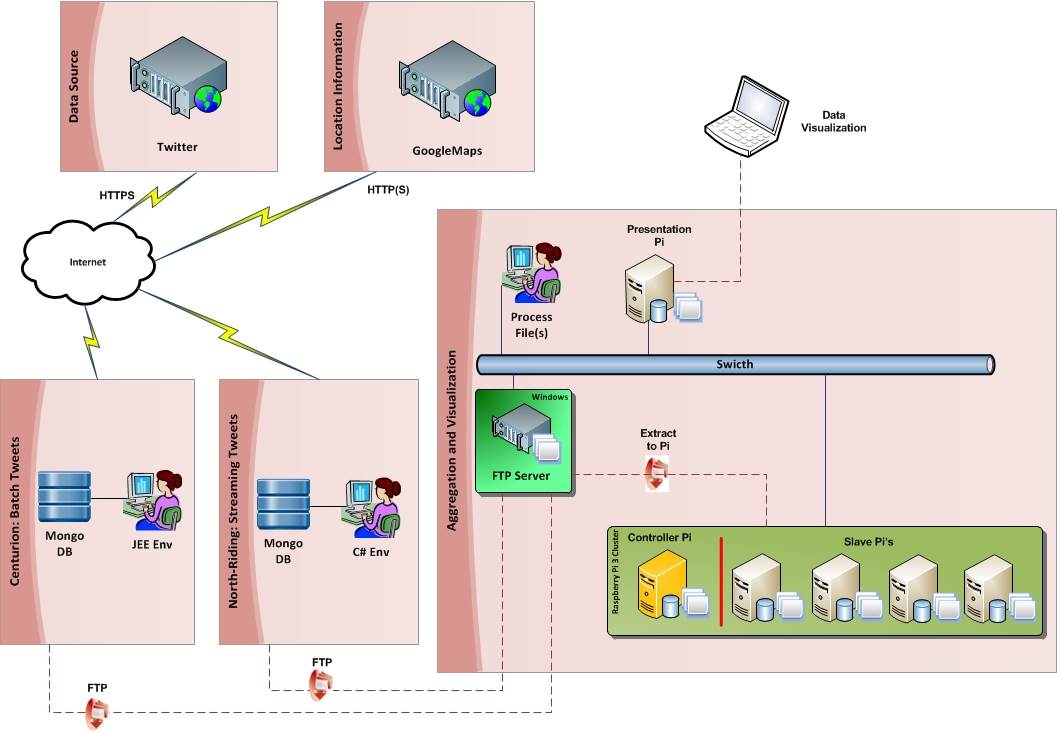
\includegraphics[width=1.15\linewidth]{OM1}}
			\caption{Operational Model: Phyical}
			\label{fig:speciation}
		\end{figure}
	
	
	\subsection{Possible Extensions}
	%\subsection{Explanation Summary} %--optional
	
	% Risk - large project given to a small company that is running a core part of the company's systems.
	
	%------------------------------------------------
	
	%\subsubsection{Executive Summary}%--optional
	
	
	%\begin{figure}[H] % Example image
	%	\center{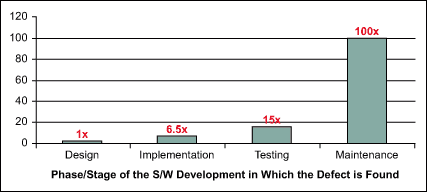
\includegraphics[width=0.55\linewidth]{IBM}}
	%	\caption{Relative Costs to Fix Software Defects (Source: IBM Systems Sciences Institute)}
	%	\label{fig:speciation}
	%\end{figure}
	
	
	
	\begin{itemize} 
		\item \textbf{Personnel Shortfall:} Inexperience in the management team is a potential risk, due to the possible oversight and inaccuracies . Leach does not have sufficient IS Management experience\textit{(pg 502 paragraph 4)}, the project may suffer if leach continues
		at his current position 
		
	\end{itemize}
	%----------------------------------------------------------------------------------------
	%	CONCLUSION
	%----------------------------------------------------------------------------------------
	
	\section{Conclusion} % Major section
	
	All this hardware and software is available to anybody interested in Big Data processing.\\
	
	The hardware is cheap and the software is free.\
	
	The learning curve in the beginning can be quite steep but is ultimately very rewarding in terms of what can be achieved with so little financial investment.
	
	
	
	
	\newpage
	
	%----------------------------------------------------------------------------------------
	%	BIBLIOGRAPHY
	%----------------------------------------------------------------------------------------
	
	\begin{thebibliography}{99} % Bibliography - this is intentionally simple in this template
		
		\bibitem 1. S. Madam. From Databases to Big Data. IEEE Computer Society, 2012.
	
		%\newblock 
		
		\bibitem 2. V. Kumar, R. Yuvaraj, C. Anusha. Effective Distribution of Large Scale Datasets Clustering Based on MapReduce. 2016.

		
	\end{thebibliography}
	
	\section{Appendices}
	
	%----------------------------------------------------------------------------------------
	
\end{document}